\chapter{Разработка программного обеспечения} \label{ch3}

\section{Проектирование архитектуры системы} \label{ch3:sec1}

Архитектура включает компоненты для сбора и хранения данных, их интеллектуального анализа, а также представления результатов и выработки корректирующих и предупреждающих действий (CAPA). На диаграмме (рис. 3.1) прямоугольниками обозначены основные модули системы, а стрелками – потоки данных и событий между ними. Сплошные стрелки отображают основной поток обработки данных от источника (репозитория) до получения результатов анализа, тогда как пунктирные стрелки показывают обмен информацией с интерактивной панелью мониторинга и инициирование действий CAPA.

\begin{figure}[ht!]
	\centering
	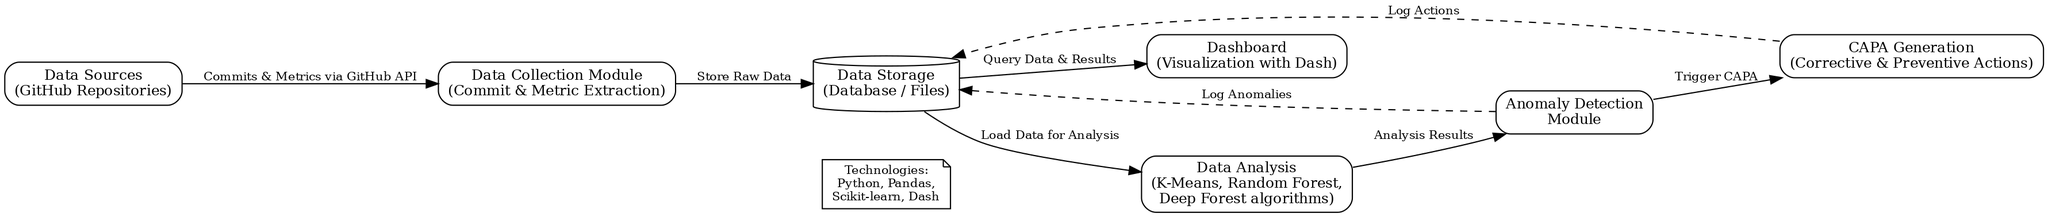
\includegraphics[width=1\textwidth]{my_folder/images/architect.png}
	\caption{Архитектура системы автоматического анализа коммитов GitHub}
	\label{fig:architecture}
\end{figure}

Основные компоненты архитектуры системы следующие:

\begin{itemize}
	\item Модуль сбора данных - отвечает за подключение к источникам данных (репозиториям GitHub) и извлечение информации о коммитах через API. Этот модуль собирает необходимые сырые данные: метаданные коммита (автор, метка времени, сообщение) и статистику изменений (количество добавленных/удалённых строк, изменённые файлы и пр.).
	\item Хранилище данных – обеспечивает сохранение полученных данных о коммитах для дальнейшей обработки. В качестве хранилища может использоваться реляционная база данных или файлы (например, CSV) в зависимости от объёма данных. Хранилище служит единой точкой, откуда аналитические модули загружают данные, а панель мониторинга получает актуальную информацию для визуализации.
	\item Модуль анализа данных – реализует обработку и анализ собранных данных с использованием методов машинного обучения. На этом этапе рассчитываются метрики коммитов (размеры изменений, сложность и др.), выполняется кластеризация (например, алгоритм k-средних) для выявления групп схожих изменений и применяется модель классификации (случайный лес, глубокий лес и др.) для определения рискованных коммитов. Результаты анализа (например, присвоенные каждому коммиту оценки риска или принадлежность к кластеру) передаются в модуль обнаружения аномалий и далее – на панель визуализации.
	\item Модуль обнаружения аномалий – специализируется на выявлении отклонений в шаблонах коммитов, в частности на аномальных временных интервалах между последовательными коммитами или нетипично крупными изменениями. Опираясь на результаты предыдущего этапа (рассчитанные метрики и кластеризацию) данный модуль идентифицирует события, выходящие за пределы нормального диапазона. Обнаруженные аномалии (например, чрезвычайно долгий промежуток между коммитами или всплеск исправлений ошибок) регистрируются и могут служить триггером для запуска процесса CAPA.
	\item Модуль генерации CAPA – формирует корректирующие и предупреждающие действия на основе выявленных проблемных ситуаций. Получая информацию о выявленной аномалии или рискованном коммите, модуль генерирует текстовые рекомендации (CAPA), направленные на исправление текущих проблем (корректирующие меры) и предотвращение подобных ситуаций в будущем (превентивные меры). Эти рекомендации могут затем автоматически фиксироваться в системе (например, добавляться в журнал действий или отправляться в виде уведомлений команде разработки).
	\item Панель визуализации (Dashboard) – интерактивное веб-приложение, реализованное с использованием фреймворка Dash, предназначено для отображения результатов анализа. Дашборд запрашивает из хранилища необходимые данные и визуализирует их в виде графиков и метрик. Он также отображает обнаруженные системой аномалии и сгенерированные рекомендации CAPA, позволяя пользователям оперативно получать информацию о состоянии проекта. Через панель разработчики могут просмотреть ключевые показатели (например, частоту коммитов, размер изменений), выявленные риски и предложенные действия по их устранению.
\end{itemize}

Предложенная архитектура обеспечивает модульность и расширяемость системы. Каждый компонент выполняет свою чётко определённую роль и взаимодействует с другими через ограниченные интерфейсы (например, совместный доступ к хранилищу или передачу сигналов об аномалиях). Такое разделение обязанностей упрощает отладку и поддержку системы, позволяя независимо совершенствовать сбор данных, аналитические алгоритмы или визуализацию. В результате спроектированная архитектура создаёт основу для эффективной реализации системы автоматического анализа коммитов и формирования CAPA.

\section{Извлечение и обработка данных из GitHub} \label{ch3:sec2}

На этапе сбора данных реализован класс GitHubRepoAnalyzer, инкапсулирующий функциональность подключения к API GitHub и анализа истории коммитов целевого репозитория. Данный класс обеспечивает получение списка коммитов, извлечение деталей каждого коммита и расчёт необходимых метрик для последующего анализа. Ниже перечислены ключевые методы и процедуры, реализованные в GitHubRepoAnalyzer:
\begin{itemize}
	\item \textbf{Аутентификация и подключение к репозиторию}. В конструкторе класса выполняется аутентификация к GitHub через токен доступа и инициализируется подключение (С помощью запросов REST API). Это позволяет в дальнейшем безопасно вызывать методы GitHub API для чтения данных.
	\item \textbf{Получение списка коммитов}. Метод \verb|fetch_commits(repo_name)| отправляет запрос к GitHub API для получения списка коммитов указанного репозитория \verb|repo_name|. Он возвращает итератор или список объектов коммитов (содержащих информацию о каждом коммите: SHA-хеш, автор, дата, сообщение, статистика изменений и др.). При необходимости данный метод может поддерживать постраничную загрузку, чтобы обработать весь исторический ряд коммитов для крупных проектов.
	\item \textbf{Извлечение данных коммита и расчёт метрик}. Для каждого коммита выполняется обработка деталей. Метод \verb|analyze_commit(commit)| рассчитывает такие показатели как: количество изменений в коде: число добавленных строк кода (additions), удалённых строк (deletions) и общее изменение (\verb|total_changes|, сумма добавленных и удалённых строк) на основе статистики диффа, предоставляемой GitHub. Затронутые файлы: число файлов, изменённых в данном коммите. Этот показатель косвенно отражает масштабы влияния изменения на кодовую базу (коммит, затрагивающий много файлов, вероятно, более комплексный). Интервал времени с предыдущего коммита: разность во времени (в днях) между текущим коммитом и предыдущим по времени. Первый коммит в истории не имеет предыдущего, для него интервал определяется как 0. Данный показатель позволяет отслеживать ритм работы над проектом. Наличие признаков багфикса: анализ текста сообщения коммита на наличие ключевых слов, указывающих на исправление ошибки (например, "fix", "bug", "error"). Если такие слова присутствуют, для коммита устанавливается флаг, что он относится к исправлению дефекта. Это служит бинарным признаком (0/1), указывающим на потенциально проблемный характер изменения (коммит, содержащий багфикс, свидетельствует о том, что ранее в коде была проблема). Оценка сложности изменения: введена дополнительная метрика сложности, оценивающая масштаб и потенциальную сложность внесённого изменения. В рамках данной работы сложность коммита приближённо характеризуется совокупностью других метрик – например, общим числом изменённых строк кода и количеством затронутых файлов. Предполагается, что коммиты с большим числом изменений и широким охватом файлов более сложны для понимания и проверки.
	\item \textbf{Сохранение и предварительная обработка}. Собранные по каждому коммиту данные сохраняются либо в оперативной памяти (в виде структуры pandas.DataFrame), либо сразу в файловое хранилище. В текущей реализации происходит запись метрик коммитов в CSV-файл (\verb|repository_data.csv|) с колонками: репозиторий, SHA коммита, автор, дата и время, сообщение, добавления, удаления, всего изменений, файлов изменено, интервал с предыдущим коммитом, признак багфикса и поле под флаг CAPA. Этот датасет затем используется на следующих этапах анализа. Перед моделированием данные могут дополнительно очищаться: устраняются дубликаты, проверяется корректность временных меток, при необходимости вычисляются дополнительные поля (например, средняя частота коммитов для автора или кумулятивные метрики).
\end{itemize}

В результате работы GitHubRepoAnalyzer формируется структурированный набор данных обо всех коммитах репозитория со значимыми характеристиками каждого изменения. Такой подход автоматизирует извлечение данных, избавляя от ручного сбора статистики, и гарантирует единообразие вычисленных метрик. Полученные данные служат основой для применения алгоритмов машинного обучения на следующем этапе. Таким образом, реализация модуля сбора и предварительного анализа данных обеспечивает подготовку качественного обучающего множества для последующего моделирования CAPA.


\section{Интеграция модели глубокого леса} \label{ch3:sec3}

Для выявления потенциально проблемных коммитов в системе используется модель классификации на основе алгоритма глубокого леса (Deep Forest). Прежде чем обучить модель, необходимо сформировать обучающую выборку, включающую признаки коммитов и целевой признак (метку), указывающую, требуется ли для данного коммита выработка CAPA. В текущей реализации разметка данных выполнена на основе эвристических правил и результатов предварительного анализа:
Коммит помечается как «требующий CAPA» (метка 1), если он удовлетворяет одному или нескольким критериям риска: например, содержит исправление ошибки (выявлено по ключевым словам в сообщении), имеет чрезвычайно большой объём изменений (значительно превышающий типичные значения по проекту) или связан с аномально долгим интервалом отсутствия активности перед ним. Такие коммиты свидетельствуют о возникновении проблем (дефект в коде, накопление большого пакета изменений, сбой в регулярности разработки), что требует принятия мер.
Коммиты, не соответствующие этим условиям, считаются обычными (метка 0). Они характеризуются типичным размером и содержанием изменений, не содержат явных признаков багфиксов и происходят с регулярной частотой, соответствующей нормальному ходу разработки.

На основе класса GitHubRepoAnalyzer из предыдущего раздела формируются признаки для модели. В качестве входных признаков (features) для каждого коммита используются:
\begin{enumerate}
	\item Общее количество изменённых строк кода (\verb|total_changes|), отражающее размер коммита.
	\item Число затронутых файлов (\verb|files_changed|).
	\item Интервал времени с предыдущего коммита (\verb|time_since_last_commit|).
	\item Наличие багфикса (булев флаг \verb|bug_fix_flag|, 1 – если в сообщении коммита обнаружены слова, указывающие на исправление ошибки).
	\item Производные или комплексные признаки сложности (например, комбинация из первых двух: большие \verb|total_changes| при большом \verb|files_changed| могут усиливать оценку сложности).
\end{enumerate}


Перед обучением количественные признаки масштабируются к сопоставимому диапазону. Если данных для обучения относительно немного, может применяться кросс-валидация или бутстреп-перемешивание для более устойчивого обучения модели. Модель глубокого леса, используемая в системе, реализована в виде классификатора CascadeForestClassifier. Данный алгоритм представляет собой каскадную композицию ансамблей решающих деревьев, альтернативный подход глубокого обучения для табличных данных. Вместо одной стадии обучения случайного леса, CascadeForest выстраивает несколько уровней (layers) из ансамблей (случайных лесов и полностью случайных деревьев), последовательно обрабатывающих данные. На каждом уровне входные признаки дополняются выходами предыдущего уровня (например, вероятностями классов), что позволяет каскаду постепенно «усложнять» представление данных и улучшать качество классификации. Обучение продолжается до тех пор, пока добавление нового уровня улучшает качество на валидационном подмножестве, либо останавливается при достижении заданного числа уровней.

В ходе обучения CascadeForestClassifier на собранных данных коммитов каждый уровень каскада строит несколько случайных лесов. Так, на первом уровне может быть обучено два случайных леса: один на исходных признаках, другой на той же выборке, но с иной инициализацией. Результаты (предсказанные вероятности классов для каждого примера) затем прикрепляются к признакам, и второй уровень обучает новые леса с расширенным пространством признаков. Такой подход позволяет модели выявлять сложные нелинейные зависимости в данных коммитов, которые мог пропустить один «плоский» алгоритм.

После тренировки модели на обучающей выборке её качество проверяется на отложенных данных (тестовом наборе) либо с помощью кросс-валидации. Оценка показала, что модель глубокого леса успешно классифицирует коммиты с точки зрения необходимости CAPA, превосходя по некоторым метрикам более простой алгоритм случайного леса. Например, для множества тестовых коммитов были корректно выявлены все случаи известных проблемных изменений при небольшом количестве ложных срабатываний.

Анализ важности признаков показал, что наибольшее влияние на решение о рискованности коммита оказывают объём внесённых изменений кода и наличие багфикса. Так, признак общего количества изменённых строк получил наивысший вес (самый информативный), поскольку крупные коммиты чаще связывались с последующими проблемами. Следующими по важности идут временной интервал (длительные паузы перед коммитом могли указывать на накопление изменений или упущенные баги) и индикатор исправления ошибок. Число затронутых файлов сыграло заметную, но меньшую роль. Анализ значимости подтверждает, что выбранные метрики обоснованно влияют на решение модели и соответствуют интуитивным представлениям: действительно, чем больше и реже изменения, тем выше вероятность необходимости дополнительных действий.

Таким образом, посредством обучения модели CascadeForestClassifier была получена интеллектуальная подсистема, способная на основе метрик коммита предсказывать необходимость CAPA. Этот классификатор служит ядром системы, автоматически оценивая каждый новый коммит и выделяя наиболее рискованные, требующие внимания разработчиков или менеджеров проекта.

\section{Реализация панели визуализации на фреймворке Dash} \label{ch3:sec4}

Визуализационная панель разработана с использованием фреймворка Dash - инструмента создания адаптивных и интерактивных веб-приложений на Python.

Интерфейс приложения разбит на несколько вкладок. Например, есть обзорная вкладка с ключевыми метриками и графиками по всем коммитам, отдельная вкладка с детальной аналитикой (графики изменений по авторам, времени и т.п.) и вкладка «Рекомендации», где в табличном виде выводится список сформированных системой корректирующих действий (CAPA) для выявленных аномалий. Для построения визуализаций используются возможности библиотеки Plotly: гистограммы (распределение числа коммитов по дням недели, авторам, величине изменений), круговые диаграммы (распределение изменений по типам или модулям), тепловые карты активности коммитов во времени и пр. Такие графики позволяют исследовать данные «вживую» и лучше выявлять закономерности

\begin{itemize} 
	\item \textbf{Структура и вкладки:} Панель разбита на тематические разделы. Например, основная вкладка показывает общее состояние репозитория (гистограммы коммитов, круговые диаграммы распределения изменений по авторам и файлам), другая – показывает детальную статистику во временном разрезе, а вкладка «Рекомендации» содержит список автоматических советов (CAPA) по улучшению процесса разработки. 
	\item \textbf{Типы визуализаций:} Используются интерактивные графики Plotly – гистограммы, круговые (pie) диаграммы, тепловые карты и линейные графики. Все эти диаграммы являются кликабельными, что позволяет пользователю изучать подробные данные.
	\item \textbf{Интерактивность:} За динамическое поведение отвечает механизм callback-функций Dash. При выборе фильтров (например, диапазона дат, конкретного автора или папки проекта) соответствующие графики автоматически обновляются.
	\item \textbf{Адаптивность интерфейса:} При создании приложения использованы компоненты \verb |dash_bootstrap_components| и тема Bootstrap. В частности, при инициализации приложения подключена тема Bootstrap (\verb|external_stylesheets=[dbc.themes.BOOTSTRAP]|), что гарантирует адаптивное размещение элементов на экране. В итоге панель корректно отображается на различных устройствах и экранах, сохраняя удобство восприятия.
	
\end{itemize}

Всё это делает дашборд удобным инструментом мониторинга: наглядные диаграммы и список рекомендаций позволяют быстро оценить состояние репозитория и принять решения на основе анализа данных.

\section{Интеграция компонентов в единую систему} \label{ch3:sec5}

Модули сбора данных, анализа и визуализации объединены в единую конвейерную цепочку обработки. Dash-приложение напрямую подключается к Python-моделям и хранилищам данных, что позволяет строить «сквозную» аналитику. В частности, Dash умеет обращаться к базам данных и другим источникам через Python-коннекторы, выполняя запросы и продвинутый анализ «на лету». роме того, фреймворк Dash хорошо интегрируется с библиотеками обработки данных (Pandas, NumPy и др.), что облегчает построение комплексных аналитических приложений.

Работа системы организована следующим образом:
\begin{itemize} 
	\item \textbf{Сбор данных:} Модуль извлечения с помощью HTTP запросов обращается к GitHub, получает историю коммитов заданных репозиториев и сохраняет её в удобном формате. Собираются метрики коммита: SHA, автор, дата, количество добавленных/удалённых строк, список затронутых файлов и т.д. Этот этап можно запускать вручную при появлении новых данных.
	 \item \textbf{Обработка и анализ:} Загруженные данные проходят первичную обработку: вычисляются дополнительные признаки (интервалы между коммитами, суммарные изменения), после чего применяется кластеризация (KMeans) для определения нормальных границ изменений. Затем обучаются модели машинного обучения Глубокого Леса для классификации коммитов на нормальные и аномальные.
	 \item \textbf{Генерация рекомендаций (CAPA):} На основе классификации система формирует корректирующие и предупредительные действия для выявленных аномалий. Для каждого «подозрительного» коммита вычисляются рекомендации (например, обратить внимание на высокую частоту изменений или большой объём кода) и при необходимости автоматически создаётся pull request с этими рекомендациями.
	 \item \textbf{Визуализация результатов:} После анализа результаты поступают на дашборд. Dash-приложение загружает актуальный набор данных (или обращается к подготовленной статистике) и отображает их в виде графиков и таблицы рекомендаций. Таким образом, пользователь получает единый интерфейс, где и графики, и текстовые CAPA-сообщения согласованы между собой.
	 \item \textbf{Автоматическое обновление:} При появлении новых коммитов цикл повторяется: система периодически выполняет сбор свежих данных, прогон анализов и обновляет панель. Пользователи получают актуальную информацию без необходимости ручного запуска каждого этапа – весь процесс сквозной автоматизации обеспечивает своевременное отображение рекомендаций и метрик.
\end{itemize}

\section{Выводы} \label{ch3:sec6}

Разработанная система была реализована в соответствии с поставленными задачами: созданы отдельные модули для извлечения данных коммитов, их анализа и визуализации. Модульный подход позволяет четко разделять функциональность и поддерживать каждый компонент независимо. 

Достигнуты ключевые цели проекта: архитектура системы является модульной и легко расширяемой – новые алгоритмы анализа или метрики могут быть добавлены без переделки остального кода. Процесс анализа коммитов полностью автоматизирован: от сбора данных до отображения результатов на панели не требуется ручного участия, что облегчает регулярный мониторинг качества разработки.  В ходе работы создан интерактивный дашборд на Dash, обеспечивающий гибкую визуализацию и удобный интерфейс для разработчиков. Это позволяет в реальном времени отслеживать состояние репозитория и эффективно использовать полученные рекомендации для улучшения кода.

Перспективы развития проекта включают расширение функционала: можно добавить новые метрики коммитов и шаблоны анализа, интегрировать систему с инструментами CI/CD и сервисами контроля качества кода, а также исследовать применение нейросетевых моделей для повышения точности предсказаний CAPA.